
\section{Resistencia aerodinámica del ala}

Conocida la curva polar de resistencia aerodinámica del perfil $\mathrm{MH}\,60$, se puede obtener la curva polar de resistencia del ala volante.

Numéricamente se calculan los coeficientes de fuerza aerodinámica para ángulos de ataque entre $-2\degrees$ y $12\degrees$ en incrementos de $1\degrees$, \ie, en el régimen de $C_L$ lineal. A partir de los vectores de $C_L$ y $C_D$, se calcula la regresión mediante una polinomio de 2º grado de $C_D = f \left( C_L \right)$. El resultado obtenido es
\begin{equation}
    C_D = 10^{-4} \left( 225.7 \, {C_L}^2 + 5.831 \, C_L + 59.44 \right)
\end{equation}
El coeficiente de término de grado 1 es un orden de magnitud inferior al término independiente y $2$ órdenes de magnitud inferior al término de grado 2. En consecuencia este se puede ignorar. La curva resultante es
\begin{equation} \label{eq:curva_polar_ala}
    C_D \approx 10^{-4} \left( 225.7 \, {C_L}^2 + 59.44 \right)
\end{equation}
por lo tanto $C_{D0} = 5.944 \cdot 10^{-3}$ y $k = 2.257 \cdot 10^{-2}$.

En la figura \ref{fig:drag_regression} se representan los resultados de la simulación numérica y la regresión de la curva de resistencia. Para $C_L$ entre $-0.2$ y $0.6$ la regresión ajusta bien a los puntos. Para $C_L > 0.6$ se aprecia cierta diferencia. No obstante, el error cometido es pequeño. 

\begin{figure}[h]
    \centering
    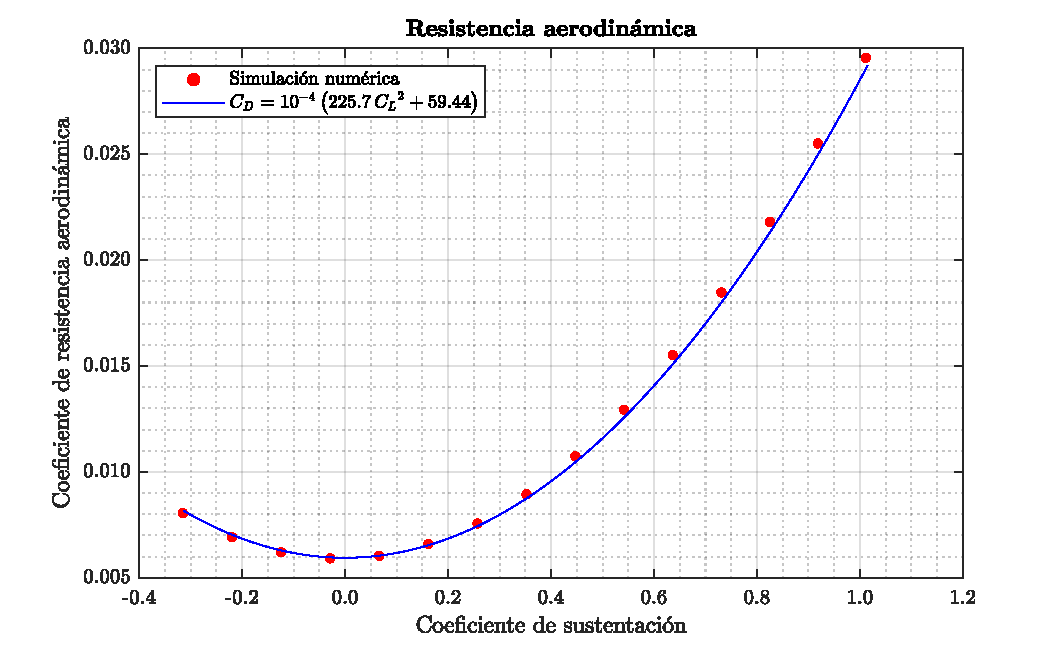
\includegraphics[width=\linewidth]{imagenes/drag_ala/drag_regression.pdf}
    \caption{Resistencia aerodinámica calculada por simulación numérica y regresión de la curva polar de resistencia.}
    \label{fig:drag_regression}
    \vspace{-4mm}
\end{figure}
